% !TeX spellcheck = en_US
\chapter{The \iceact Model in \geant}

The optical system of \iceact is modeled in \geant. The following chapter will give a view on the material properties and working principles on all optical components.

\section{\geant}

\begin{wrapfigure}{r}{0.5\textwidth}
	\centering
	
\includegraphics[width=0.5\textwidth]{Geant4Logo.png}
	\caption[\geant logo]{\textbf{\geant logo.} \cite{geant4:logo}}	
\end{wrapfigure}
\geant is a multi-purpose simulation framework for the passage of particles trough matter, written in \textit{C++} and developed by the \geant Collaboration at CERN. It includes physics models, geometry, tracking, hits, and digitization. Thus, it allows detailed simulations and response analyses for particle detectors in many application fields like particle and accelerator physics, space engineering or medical science. In the framework's source some basic and advanced use cases are implemented and provided as examples. The toolkit is built up of multiple categories (or modules) using each other (cf. figure \ref{geant4:categories}).~\cite{geant4}

\begin{figure}[H]
	\centering
	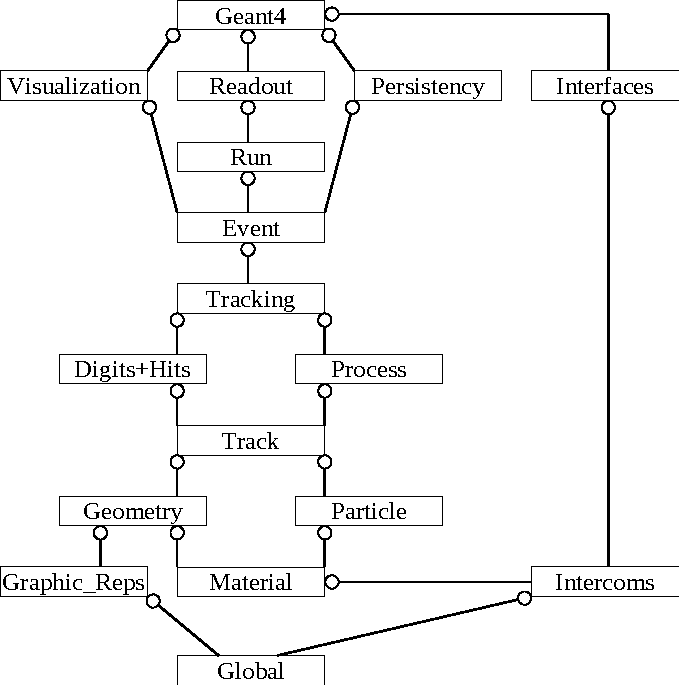
\includegraphics[width=0.5\textwidth]{Geant4ConceptDiagram.pdf}
	\caption[\geant category diagram]{\textbf{Diagram of relationships between \geant categories.} \cite[adapted]{geant4} The circles represent a \enquote{using} relation. The category with the circle next to the box uses the linked one.}	
	\label{geant4:categories}
\end{figure}

Especially for \iceact, \geant is capable of simulating Cherenkov (optical) photons, material properties like transmission, reflection, and refraction, as well as detection efficiency properties of the SiPMs.

Since this thesis is about an approach of an all-encompassing telescope simulation, \geant provides all major possibilities to get a distinct analysis of the entire optical system of \iceact.

\subsection{FAMOUS telescope simulation}\label{sec:famous_simulation}
The fluorescence telescope FAMOUS\footnote{\textbf{F}irst \textbf{A}uger \textbf{M}ulti-pixel
photon counter camera for the \textbf{O}bservation of \textbf{U}ltra-high-energy air \textbf{S}howers} for the Pierre Auger Observatory in Argentina is developed at RWTH Aachen to measure fluorescence light originating from ultra-high-energy cosmic rays (UHECR) by using Silicon Photomultipliers (SiPMs). Within the development, a detailed \geant simulation has been elaborated \cite{famous:sim_github,famous:sim_github}. The telescope design of FAMOUS is similar since the detection technique and the optics system is basically the same. Therefore, the \iceact telescope simulation is based on this FAMOUS \geant framework. A detailed discourse and a summary of previous analyses can be found in~\cite{famous:niggemann}.

\section{Materials}\label{sec:iceact:model:material}

For an optical device, the material that the light should pass has to be chosen deliberately. Especially the transmission properties, processability, and for \iceact in particular the resistance against harsh weather conditions are of interest.\\

The glass plate on top of \iceact is made of SCHOTT BOROFLOAT\textsuperscript{\textregistered} 33 borosilicate glass. Borosilicate is chosen for its high durability, transparency in the interesting spectral region, flatness, and weak fluorescence intensities. The refractive index is evaluated at some wavelength. Since we need to have a full dispersion relation the points are spline interpolated (cf. orange curve in figure~\ref{iceact:model:material:refractive_index}).~\cite{iceact:borosilicate:datasheet}

In the BOROFLOAT\textsuperscript{\textregistered} 33 data sheet~\cite{iceact:borosilicate:datasheet} the transmission properties are given for a vertical light and a glass plate of a thickness of $d = \SI{6.5}{\milli\meter}$. Therefore, the transmission curve $T_\text{total}(\lambda)$ includes the internal absorption as well as the two interface transitions into and out of the borosilicate which yields
\begin{align}
	T_\text{total}(\lambda) = T_\text{interface}^2(\lambda)\cdot T_\text{internal}(d=\SI{6.5}{\milli\meter},\lambda)\,.
	\label{eq:transmission}
\end{align}
The transmission at the interface can be calculated by using the Fresnel equations \cite{fresnel_equations}. In case of perpendicular light, it is
\begin{align}
	T_\text{interface}(\lambda) = 1 - \left(\frac{n(\lambda)-n_\text{air}}{n(\lambda)+n_\text{air}}\right)^2\,.
	\label{eq:perp_interface_transmission}
\end{align}
In \geant the wavelength dependent absorption length $a(\lambda)$ has to be implemented which is given by exponential absorption:
\begin{align}
	I(x) = I_0 e^{-\frac{x}{a}} \Leftrightarrow a = - \frac{x}{\ln{\frac{I(x)}{I_0}}}\,.
	\label{eq:absorptionlaw}
\end{align}
Thus, one gets the absorption length by using equations~\eqref{eq:transmission}, \eqref{eq:perp_interface_transmission}, and \eqref{eq:absorptionlaw} with
\begin{align}
	a(\lambda) &= - \frac{d}{\ln T_\text{internal}(d,\lambda)}\nonumber\\
	&= \frac{d}{2\ln\left(1 - \left(\frac{n(\lambda)-n_\text{air}}{n(\lambda)+n_\text{air}}\right)^2\right)-\ln T_\text{total}(\lambda)}\,.
\end{align}
This is implemented in the \geant material properties with $n_\text{air} = 1$. Figure \ref{iceact:model:material:transmission} shows the three transmission components as orange lines.\\

The Fresnel lens and the Winston Cones in \iceact are made of polymethyl methacrylate (PMMA). The dispersion~$n(\lambda)$ can be parametrized with the empirical \textit{Sellmeier equation}~\cite{iceact:sellmeier}. For glasses, the usual form is
\begin{align}
	n^2(\lambda) = 1 + \frac{B_1\lambda^2}{\lambda^2-C_1} + \frac{B_2\lambda^2}{\lambda^2-C_2} + \frac{B_3\lambda^2}{\lambda^2-C_3}\,,
	\label{eq:sellmeier}
\end{align}
with the \textit{Sellmeier coefficients} $B_{1,2,3}$ and $C_{1,2,3}$~\cite{iceact:sellmeier}. Table~\ref{iceact:model:pmma_sellmeiercoeffs} shows the used coefficients and the function is plotted in figure~\ref{iceact:model:material:refractive_index} (blue curve).

\begin{table}[H]
	\centering
	\begin{tabular}{c|l}
		$B_1$  & \num{0.99654}  \\
		$B_2$  & \num{0.18964}  \\
		$B_3$  & \num{0.00411}  \\
		$C_1$  & \SI{0.00787}{\micro\meter\squared}  \\
		$C_2$  & \SI{0.02191}{\micro\meter\squared}  \\
		$C_3$  & \SI{3.85727}{\micro\meter\squared}  \\
	\end{tabular}
	\caption[Sellmeier coefficients for PMMA]{\textbf{Sellmeier coefficients for PMMA.}~\cite{iceact:refractiveindex} The above-mentioned coefficients are used in the \geant material properties for PMMA. The related Sellmeier equation~\eqref{eq:sellmeier} is plotted in figure \ref{iceact:model:material:refractive_index} as the blue curve.}
	\label{iceact:model:pmma_sellmeiercoeffs}
\end{table}

For the transmission properties of PMMA, the same method as for borosilicate is used (see above). Therefore, the data stated in \cite{famous:niggemann} is taken as $T_\text{internal}(d = \SI{3}{\milli\meter})$. Figure \ref{iceact:model:material:transmission} shows the three transmission components as blue lines.

\begin{figure}[H]
	\centering
	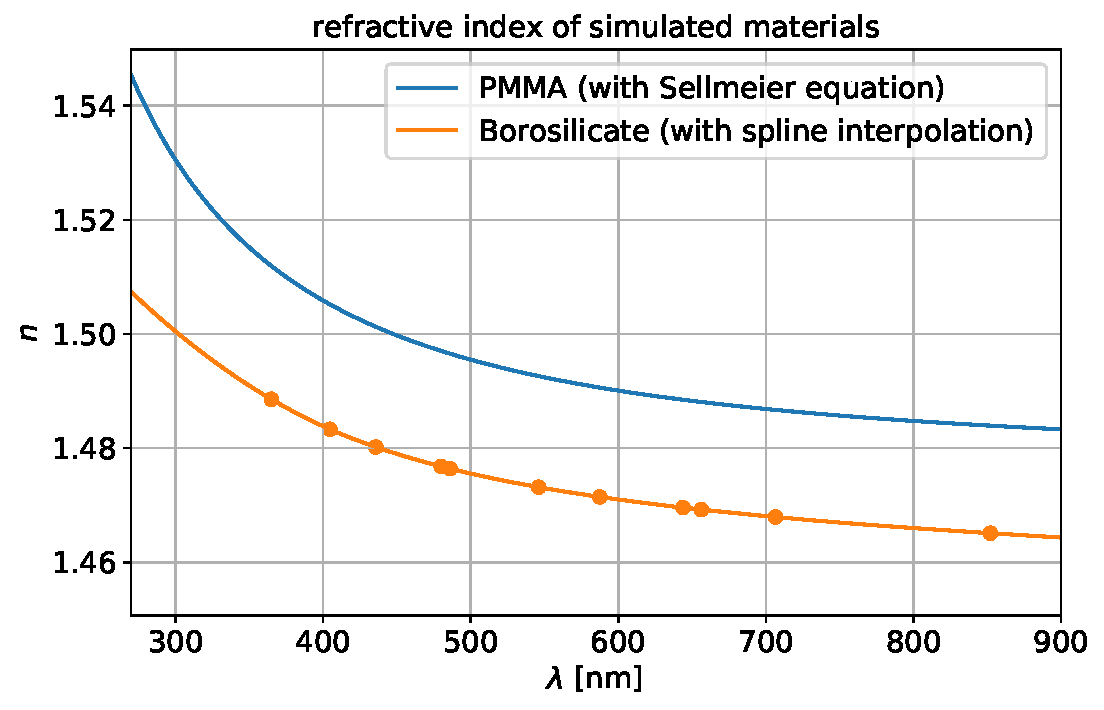
\includegraphics[width=0.7\textwidth]{material/refractive_index.pdf}
	\caption[Refractive index of used materials]{\textbf{Refractive index of materials used in the simulation.} For PMMA the dispersion is calculated by evaluating the Sellmeier equation introduced in this section. The refractive index for the used borosilicate is only given for specific wavelengths \cite{iceact:borosilicate:datasheet}. Therefore, splines are used to inter- and extrapolate the full curve.}
	\label{iceact:model:material:refractive_index}	
\end{figure}

\begin{figure}[H]
	\centering
	\begin{subfigure}[t]{0.485\textwidth}
		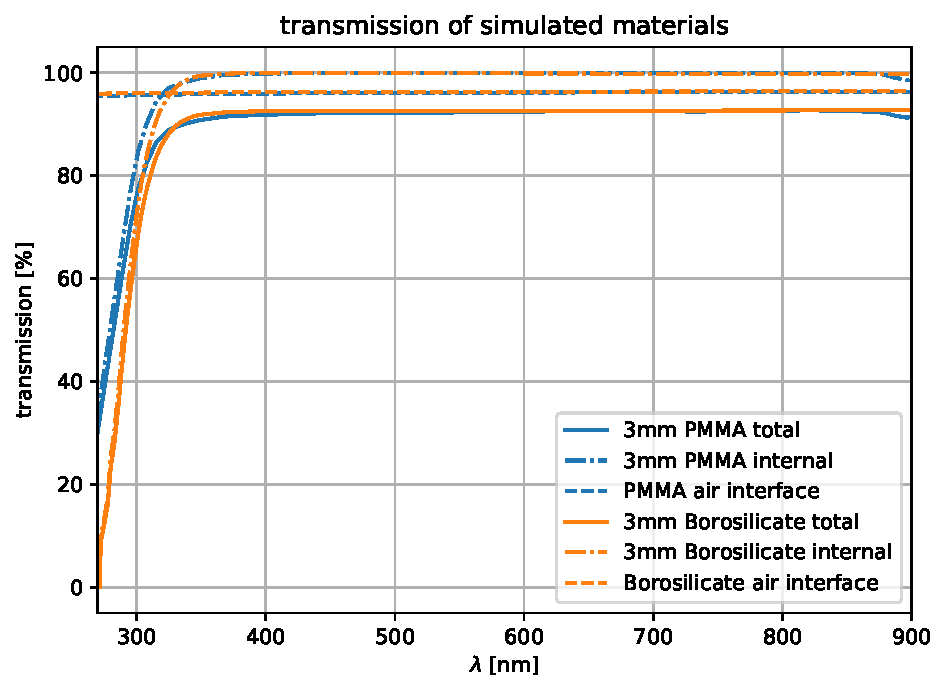
\includegraphics[width=\textwidth]{material/transmission.pdf}
		\subcaption{full view}
	\end{subfigure}
	\hfill
	\begin{subfigure}[t]{0.499\textwidth}
		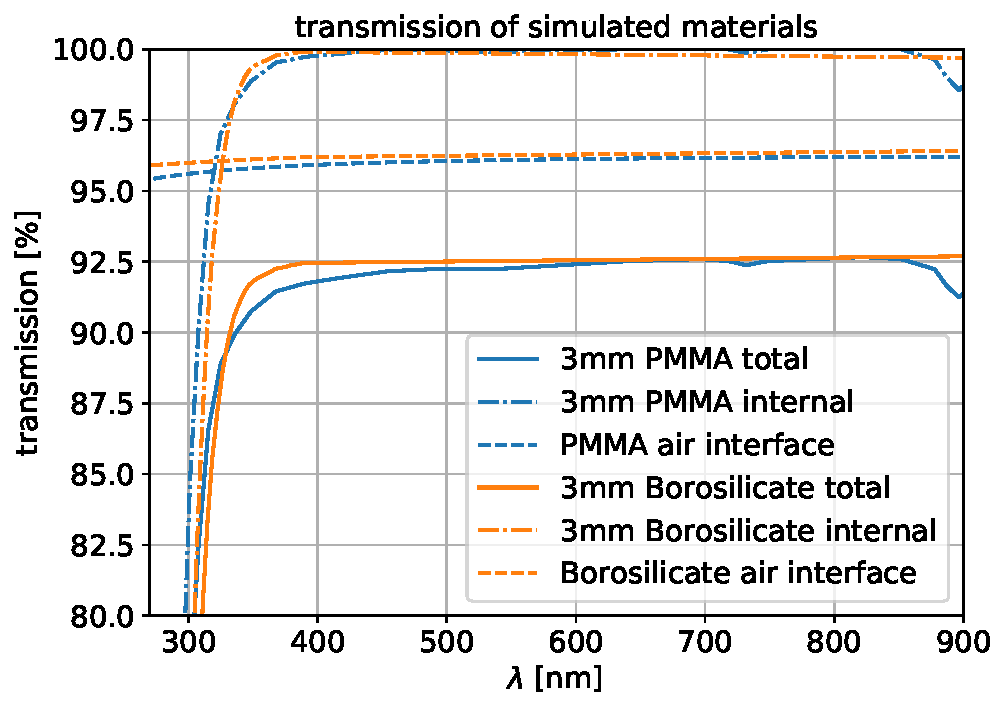
\includegraphics[width=\textwidth]{material/transmission_zoom.pdf}
		\subcaption{zoomed view}
	\end{subfigure}
	\caption[Transmission of used materials]{\textbf{Transmission functions of materials used in the simulation.} The total transmission function is the product of internal and two interface transmissions which is evaluated for a perpendicularly incident particle in this plot. Thus, the solid lines represent a complete (perpendicular) transition through a $d=\SI{3}{\milli\meter}$ thick layer of the respective material. For a better comparison, the data of internal transmission for borosilicate (given for $d=\SI{6.5}{\milli\meter}$ in~\cite{iceact:borosilicate:datasheet}) is converted for  $d=\SI{3}{\milli\meter}$.}
	\label{iceact:model:material:transmission}	
\end{figure}

The tube, back plane and other coating surfaces are simulated as \enquote{dummy} material with no reflection or transmission parameters. A particle that hits those surfaces is absorbed and not considered any further.

\section{Optics}

As introduced in section \ref{sec:iceact_intro}, \iceact is designed to image the direction of Cherenkov light on a camera consisting of multiple pixels. The imaging is done by a Fresnel lens, and an SiPM-based camera with light collecting \enquote{cones}. A sketch of the camera layout is shown in figure \ref{iceact:camera:layout}
\begin{figure}[H]
	\centering
	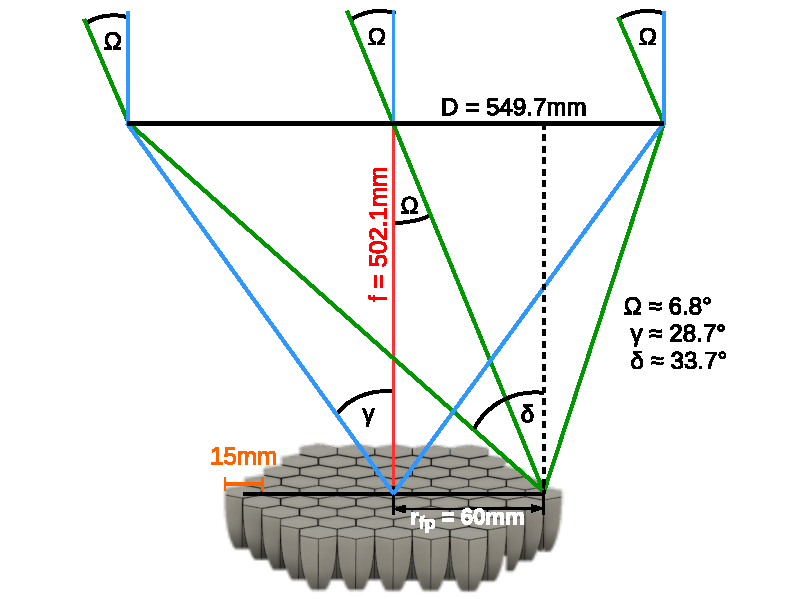
\includegraphics[width=0.6\textwidth]{CameraDesign.pdf}
	\caption[\iceact camera layout]{\textbf{The \iceact camera layout.} \cite{iceact:camera} In this sketch the Fresnel lens with a diameter $D=\SI{549.7}{\milli\meter}$ and a focal length of $f=\SI{502.1}{\milli\meter}$ focusing rays to the camera sketched below. Additionally, three characteristic angles are shown: the maximum incidence angle of a ray to be focused on the camera plane $\Omega\approx\SI{6.8}{\degree}$, the maximum incidence angle on the central Winston cone $\gamma\approx\SI{28.7}{\degree}$, and the maximum incidence angle for the outermost Winston cone $\delta\approx\SI{33.7}{\degree}$.}
	\label{iceact:camera:layout}	
\end{figure}

In the following section the four optical components of the \iceact \geant model are discussed. Figure~\ref{iceact:model:cut} shows a cross-sectional sketch of the model.
\begin{figure}[H]
	\centering
	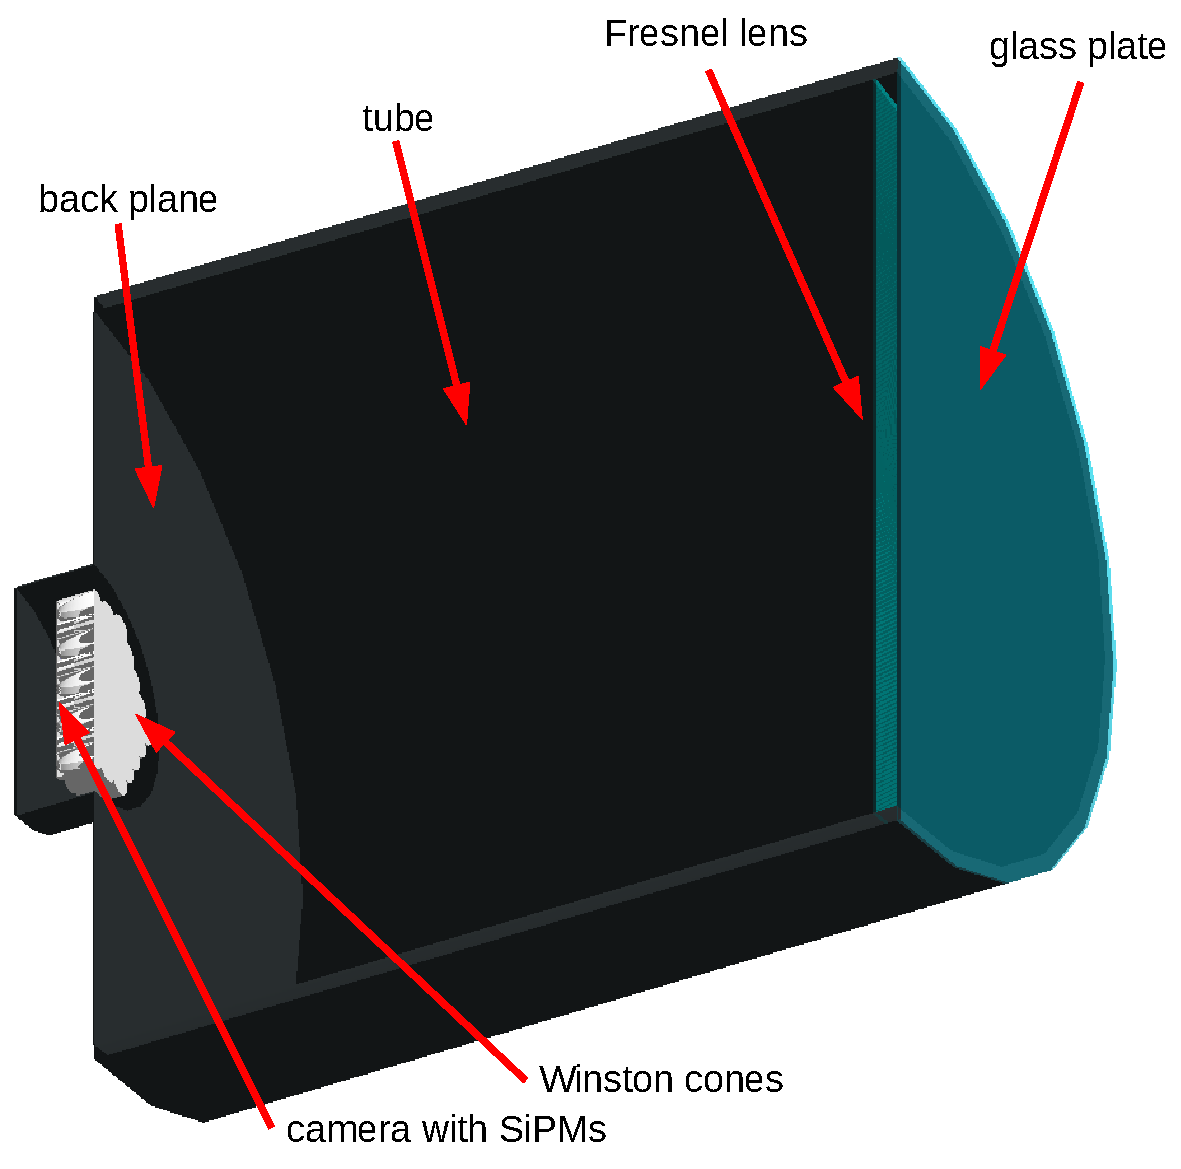
\includegraphics[width=0.6\textwidth]{IceActGeant4Model.pdf}
	\caption[\iceact \geant model]{\textbf{The \iceact \geant model.} Cross-sectional sketch of the \iceact optics in \geant with all simulated components. They are described in detail in \cref{iceact:model:fresnellens,iceact:model:camera,iceact:model:glassplate}.}
	\label{iceact:model:cut}	
\end{figure}

\subsection{Glass Plate}\label{iceact:model:glassplate}

The \iceact glass plate has a thickness of \SI{2+-0.2}{\milli\meter}, a diameter of \SI{650.3+-1}{\milli\meter}, and is made of borosilicate as mentioned in section~\ref{sec:iceact:model:material}. It is mounted on top of the tube and its major purpose is to protect the Fresnel lens from the environment. At South Pole conditions, one of the major challenges for the optical system is adherence of snow above the lens which reduces the field of view. In the \SI{12.2}{\milli\meter} thick air gap between glass plate and Fresnel lens a heating cable is installed to remove snow from the glass surface. 

\subsection{Fresnel Lens}\label{iceact:model:fresnellens}

The two major advantages using a Fresnel lens rather than a conventional lens are the significantly less weight and the fact that light passes less material which could absorb it. The main idea of a Fresnel lens is to divide a thick lens into small annular facets in form of prisms that keep the local inclination of the conventional lens by making local approximations of the lens' \textit{sagitta function}\footnote{In application to lenses, the sagitta function~$z(\rho)$ gives the lens thickness $z$ as a function of the radial distance $\rho$ from the optical axis for radially symmetrical lenses.}. Figure~\ref{iceact:model:fresnelvsthick} visualizes the principle. \iceact uses the model ORAFOL SC 943 with an aperture of \SI{549.7}{\milli\meter}, a focal length of \SI{502.1}{\milli\meter} at a wavelength of \SI{546+-27.3}{\nano\meter}. The lens is \SI{2.5}{\milli\meter} thick, has 10 grooves per \si{\milli\meter}, and is made of polymethyl methacrylate (PMMA) as stated in section~\ref{sec:iceact:model:material}.~\cite{iceact:fresnellens:datasheet}

\begin{figure}[H]
	\centering
	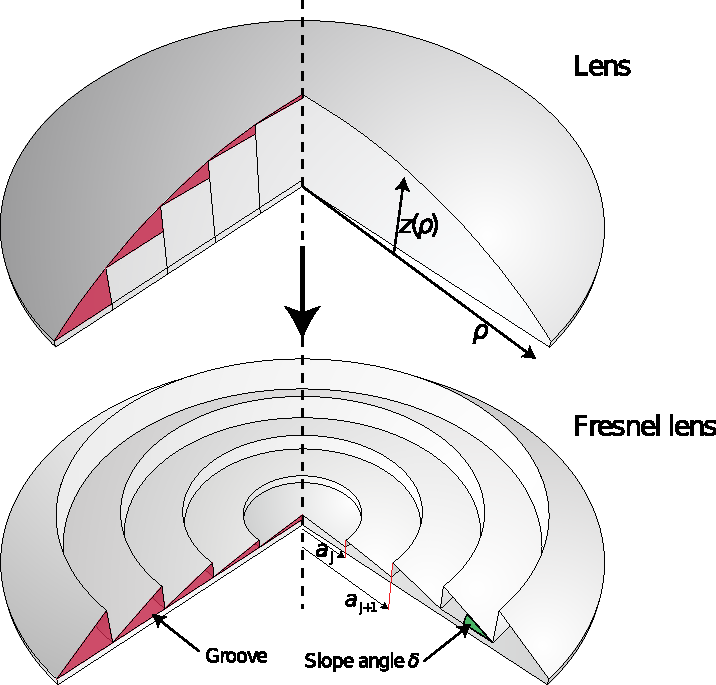
\includegraphics[width=0.5\textwidth]{FresnelVsNormalLens.pdf}
	\caption[Comparison conventional vs. Fresnel lens]{\textbf{Comparison between a conventional \enquote{thick} lens and a Fresnel lens.} \cite{famous:eichler} For the functionality of a lens the radius-dependent sagitta function $z(\rho)$ is crucial. To get rid of the bulky material of a conventional lens, the Fresnel lens is divided into annular \enquote{prisms} called \enquote{grooves}. The slope angle $\delta$ of each groove is a local approximation of the sagitta function to ensure the imaging capability.}
	\label{iceact:model:fresnelvsthick}	
\end{figure}

\begin{figure}[H]
	\centering
	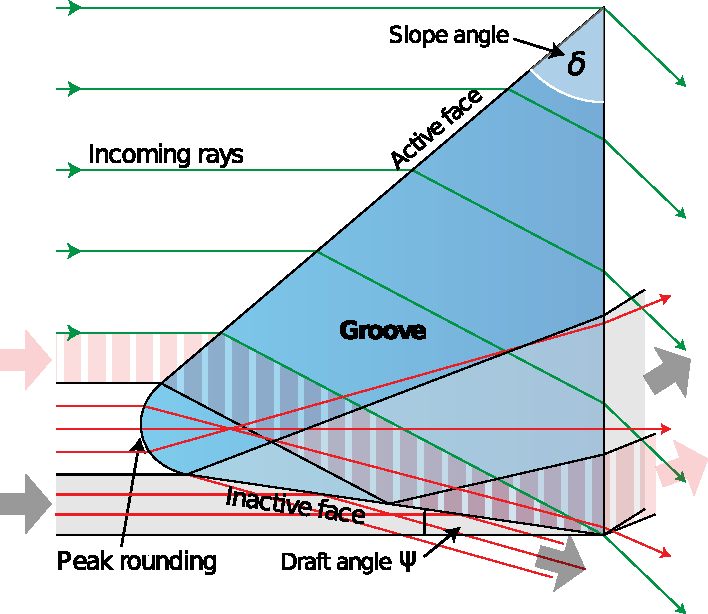
\includegraphics[width=0.5\textwidth]{FresnelGroove.pdf}
	\caption[Fresnel groove]{\textbf{Cross-sectional sketch of a Fresnel groove.} \cite{famous:eichler} Most of the incoming rays are hitting the regular active (or slope) facet of the groove with slope angle $\delta$. For an optimal groove, the inactive (or draft) facet would be parallel to the optical axis. Due to manufacturing process, there is always a small slope on the inactive facet given by the draft angle $\psi$ and the peak is rounded. With this design, there are some impact regions where incoming rays are not refracted to the focal point: if they undergo total reflection at the inactive facet inside the groove (red-dashed region), if they hit the peak rounding (red rays), or if they hit the inactive face (gray region).}
	\label{iceact:model:fresnelgroove}	
\end{figure}

\begin{figure}[H]
	\centering
	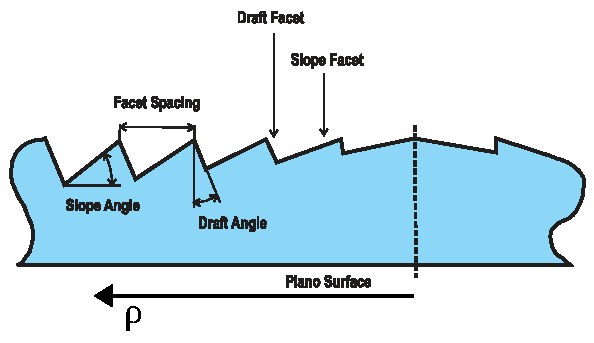
\includegraphics[width=0.5\textwidth]{FresnelSideProfile.pdf}
	\caption[Fresnel side-profile]{\textbf{Side-profile sketch of a Fresnel lens.} \cite[adapted]{iceact:fresnellens:design}. Complementary sketch to figure \ref{iceact:model:fresnelgroove} which shows the draft angle increase with radius $\rho$ driven by manufacturing.}
	\label{iceact:model:fresnelprofile}	
\end{figure}

The transmission of a Fresnel lens is not just given by the material properties. Due to the groove structure there are so called \textit{draft facets} where unwanted refractions, reflections, or transmissions occur. One can compensate for this by adjust the \text{draft angle} $\psi$ (cf. figures \ref{iceact:model:fresnelgroove} and \ref{iceact:model:fresnelprofile}) as a function of the lens radius $\rho$. Anyway, the molding process -- which is the common manufacturing technique of Fresnel lenses -- does not allow to have a perpendicular draft facet ($\psi = 0$) due to mold release. This forces the lens to have a minimum draft angle of $\psi_0 = \SI{3}{\degree}$. With the optimization mentioned before, this leads to a radial dependent draft angle which can be expressed as \cite{famous:eichler, famous:niggemann}
\begin{align}
	\psi(\rho) = \SI{3}{\degree} + \SI{0.0473}{\degree\per\milli\meter}\rho\,.
\end{align}
This draft angle function is implemented in the Fresnel lens design in \geant, the groove peak rounding suggested in figure~\ref{iceact:model:fresnelgroove} is not. The effect of simulating the rounding is discussed in \cite{famous:eichler} with the result that a peak rounding radius of $\SI{5}{\micro\meter}$ would slightly enlarge the aberration radius by a few \SI{10}{\micro\meter}.

Nevertheless, one has to be aware of the fact that approximating a thick lens by a Fresnel lens comes along with losses due to those \enquote{false} optical projections and results in aberration effects. A detailed discussion and measurement of point spread functions and optical aberrations is done in \cite{famous:niggemann} and \cite{famous:eichler}.

\subsection{Camera}\label{iceact:model:camera}

\begin{figure}[H]
	\centering
	\saveimageheight[width=0.49\textwidth]{SiPMs.pdf}
	\begin{subfigure}[t]{0.49\textwidth}
		\raiseimage[width=\textwidth]{Camera.png}
		\subcaption{Picture of the assembled \iceact camera.~\cite{iceact:camera:burgmann} 61 \enquote{hex-to-square} Winston cones are glued onto the hexagonal SiPM grid. Besides, one can see two of the overall three additional pixels for reference measurements.}
		\label{iceact:camera:picture}	
	\end{subfigure}
	\hfill
	\begin{subfigure}[t]{0.49\textwidth}
		\usebox{\savedimage}
		\subcaption{Placing sketch and pixel numbering of the camera where the 61 pixels are numbered in a spiral scheme starting with the central pixel with the \geant coordinate system. In the hexagonal grid all SiPM centers have a distance of \SI{15}{\milli\meter} to their next neighboring pixels. The bright blue SiPMs are \enquote{open} pixels without a Winston cone on top and the dark blue SiPM is a \enquote{blind} pixel.}
		\label{iceact:camera:pixelnumbering}	
	\end{subfigure}
	\caption[The \iceact camera]{\textbf{The \iceact camera.}}	
\end{figure}

The \iceact camera is the compound of 61 Silicon Photomultipliers (SiPMs, cf. section~\ref{sec:sipm_working_principle}) arranged in a hexagonal grid together with 61 Winston cones (cf. section~\ref{sec:winstoncones}) glued on them. In addition to the 61 instrumented pixels there are three pixels aside for reference measurements. Two of them are just placed without Winston cones on top to measure optical noise while one pixel is completely \enquote{blind} by being masked. This makes it possible to measure the pure electronic noise of the SiPM. Figure~\ref{iceact:camera:picture} shows an assembled \iceact camera. To address each pixel, they are numbered in a spiral scheme starting with the central \enquote{0$\text{th}$} pixel and going outside counterclockwise as seen from the top (cf. figure~\ref{iceact:camera:pixelnumbering}).\\

In the following sections, the working principle as well as the implementation in \geant is discussed.

\subsubsection{Winston Cones -- Working Principle}\label{sec:winstoncones}

\begin{wrapfigure}{r}{0.5 \textwidth}
	\centering
	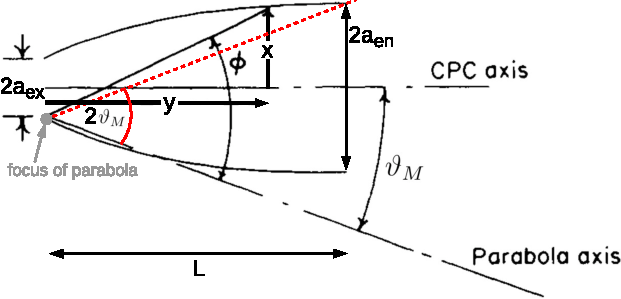
\includegraphics[width=0.5\textwidth]{WinstonConeSketch.pdf}
	\caption[Sketch of a Winston cone]{\textbf{Sketch of a Winston cone.} \cite{iceact:camera} The shape of the cone is given by the two sketched parabolic curves rotating around the CPC axis. Characteristic lengths and angles are indicated: the entrance and exit diameters $a_\text{en,ex}$, the cone length $L$, the maximum incidence angle $\vartheta_\text{M}$, the parameterization coordinates $(x,y)$, and the angle $\phi\in[\vartheta_\text{M},\vartheta_M+\SI{90}{\degree}]$ needed for parameterization as well.}
	\label{iceact:camera:wico_sketch}	
\end{wrapfigure}

The \iceact telescopes use a light collection technique to enlarge the detection area of the SiPM grid based on \textit{compound parabolic concentrators} (CPC) \cite{wico:book}. In the following, this concentrators are named \textit{Winston cones}. 
Primarily, a Winston cone is a rotationally symmetrical paraboloid formed by an off-axis parabola revolving around the axis of symmetry (\textit{CPC axis}, cf. figure \ref{iceact:camera:wico_sketch}). Hence, the entrance area $A_\text{en}=\pi a_\text{en}^2$ and the exit area $A_\text{ex}=\pi a_\text{ex}^2$ are circular. The concentration effect works for every ray hitting the entrance area up to the maximum angle $\vartheta_\text{M}$. A relation between $\vartheta_M$ and the characteristic lengths shown in figure~\ref{iceact:camera:wico_sketch} can be found: \cite{wico:book,iceact:camera}
\begin{align}
	\sin\vartheta_\text{M} = n\cdot\frac{a_\text{ex}}{a_\text{en}}\,,
	\label{eq:wico:theta_max}
\end{align}
with the refractive index $n$ of the cone material. The appearance of the refractive index connotes the to major working principles of Winston cones. On the one hand, light can be concentrated by using surface reflections in hollow cones ($n=n_\text{air}\approx 1$), or -- on the other hand -- using internal total reflections in solid cones ($n>1$). Equation~\eqref{eq:wico:theta_max} shows that the maximum angle can be increased by using a solid cone with a preferably large refractive index.

The parabola describing the Winston cone surface is further called \textit{Winston curve} and can be parameterized by \cite{wico:book,iceact:camera}
\begin{subequations}
	\label{eq:wico:param}
	\begin{align}
	x &= \frac{2a_\text{ex}(1+\sin\vartheta_\text{M})\sin(\phi-\vartheta_\text{M})}{1-\cos\phi}-a_\text{ex}\,,\\
	y &= \frac{2a_\text{ex}(1+\sin\vartheta_\text{M})\cos(\phi-\vartheta_\text{M})}{1-\cos\phi}\,,
	\end{align}
\end{subequations}

with the cone radius $x$, the cone length $y$, and the angle $\phi$ between the connecting line of focus of parabola and a point on the opposite parabola and the parabola axis (cf. figure~\ref{iceact:camera:wico_sketch}).

Another important quantity is the cone length $L$ which is given by \cite{wico:book,iceact:camera}
\begin{align}
	L = \frac{a_\text{ex}(1+\sin\vartheta_\text{M})\cos\vartheta_\text{M}}{\sin^2\vartheta_\text{M}}\sim\frac{2a_\text{en}}{2\vartheta_\text{M}}\,.
\end{align}






By appropriate design, Winston cones fulfill all requirements for light concentrators in \iceact given by the optical layout (cf. figure~\ref{iceact:camera:layout}).
However, one can design an improved Winston cone for the purposes in \iceact since a hexagonal grid of quadratic pixels with an area of $\SI{6}{\milli\meter}\times\SI{6}{\milli\meter}$ is used (cf. figure~\ref{iceact:camera:pixelnumbering}). Instead of a radially symmetrical cone, the \iceact Winston cone is designed in such a way that the exit window fits the SiPM area while the entrance window is hexagonal to maximize the camera's detectional area (cf. figure~\ref{iceact:camera:picture}). This design is called \textit{hex-to-square}. A sketch of the \iceact Winston cone is shown in figure~\ref{iceact:camera:iceact_wico_sketch}. In it, one can see a green dashed line and a pink solid line on the cone's side which follow optimized Winston curves by using the parameterization of equations~\eqref{eq:wico:param}.

\begin{figure}[H]
	\centering
	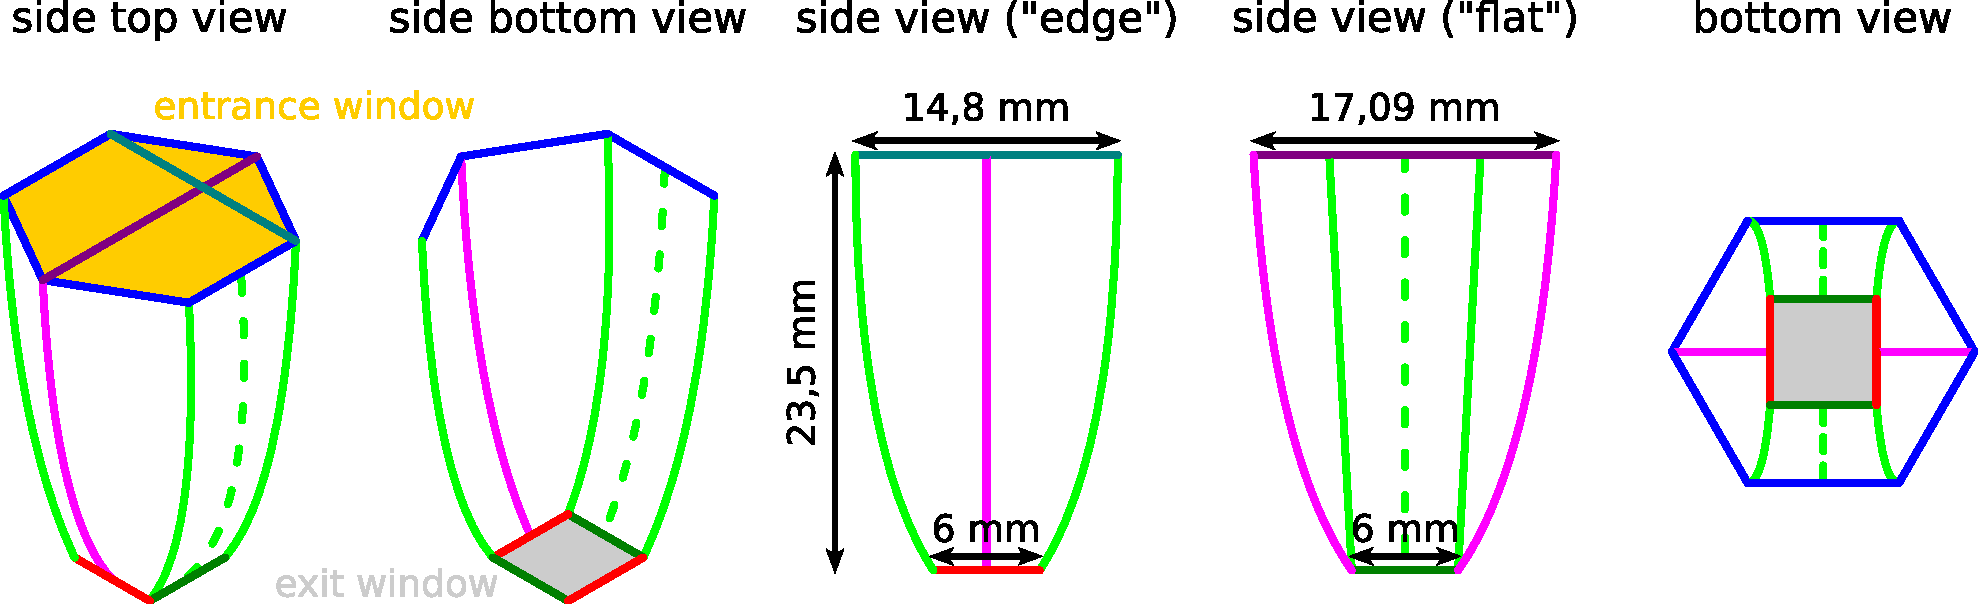
\includegraphics[width=\textwidth]{IceActWiCoSketches.pdf}
	\caption[Sketches of the \iceact \enquote{hex-to-square} Winston cone]{\textbf{Sketches of the \iceact \enquote{hex-to-square} Winston cone.} The cone is shown from different points of view with dimensioning. The pink edge and the green dashed surface line follow the optimized Winston curve functions developed in \cite{iceact:camera}. The green dashed curve is extruded in order to form the whole side. Two different functions result in two different maximum angles $\vartheta_\text{M}^\text{edge,side}$ for an incidence parallel to the \enquote{edge} or the \enquote{side} plane.}
	\label{iceact:camera:iceact_wico_sketch}	
\end{figure}

Hence, the application of Winston cones extend the detectional area of the pixels by a factor of (cf. figure \ref{iceact:camera:iceact_wico_sketch})
\begin{align}
	\frac{A_\text{camera with WiCos}}{A_\text{camera without WiCos}} = \frac{61\cdot \frac{3}{2}\sqrt{3}\cdot\left(\frac{\SI{17.09}{\milli\meter}}{2}\right)^2}{61\cdot(\SI{6}{\milli\meter})^2}\approx\num{5.27}\,.
\end{align}

\subsubsection{Winston Cone Implementation in \geant with CADMesh}

Due to its complex shape the cones are implemented in \geant by decomposing their CAD\footnote{\textbf{C}omputer-\textbf{a}ided \textbf{D}esign, technique to use a computer for the creation, analysis, etc. of a design.} sketch into small triangular tiles called \textit{meshing}. For the \iceact Winston cone this is done with the CAD software \textit{FreeCAD}, more precisely with the algorithm \textit{Mefisto}. This meshing routine only needs the maximum edge length of the single tiles as a free parameter. The smaller the maximum edge length the more detailed the mesh gets but the more computational time is needed to translate this mesh into \geant. Thus, a good compromise has to be found. Figure~\ref{wico:meshing} shows the meshed cone dependent on the maximum edge length. Simulations show a good performance for a maximum egde length of \SI{0.2}{\milli\meter}. Higher lengths result in visible image artifacts. (cf. section~\ref{sec:wico_meshing}) 

\begin{figure}[H]
	\centering
	\includegraphics[width=\textwidth]{wicomeshes/WiCo_Meshes.pdf}
	\caption[\iceact Winston cone meshing with different maximum edge lengths]{\textbf{\iceact Winston cone meshing with different maximum edge lengths.} The accuracy increases by reducing the maximum edge length of the tiles. The length of \SI{0.2}{\milli\meter} is used in the simulation.}
	\label{wico:meshing}	
\end{figure}

The meshed geometry is then translated into \geant by using the toolkit \textit{CADMesh} \cite{wico:cadmesh}. More about Winston cone meshing is discussed in section \ref{sec:wico_meshing}.

\subsubsection{Silicon Photomultipliers (SiPM)}\label{sec:sipm:working_principle}

Silicon Photomultipliers (\textit{SiPM}s) are semiconductor devices used for photon detection in multiple applications. In comparison to conventional photon detection devices like Photomultiplier Tubes (\textit{PMT}s) they are rather compact and offer a higher detection efficiency. These features made them interesting devices for application in imaging detectors.

An SiPM is the composition of an array of so called \textit{Geiger-mode avalanche photo diodes} (\mbox{\textit{G-APD}s}). Their working principle is based on $p$-$n$-junctions (cf. figure~\ref{sipm:pn_junction}). This is the simple configuration when an $n$-doped and a $p$-doped material are brought together. Thus, a \textit{depletion zone} occurs where free electrons of the $n$-doped material fill holes of the $p$-doped material. Due to the resulting net charge, an electric field arises from the $n$- to the $p$-doped side, comparable to a capacitor. The size of the depletion zone can be enlarged by an external \textit{bias voltage} $V_\text{bias}$ applied with the anode side at the $n$-doped material. In this state, the junction conducts current easily only in one direction, which is commonly known as a \textit{diode}. \cite{pn:simon}

\begin{figure}[H]
	\centering
	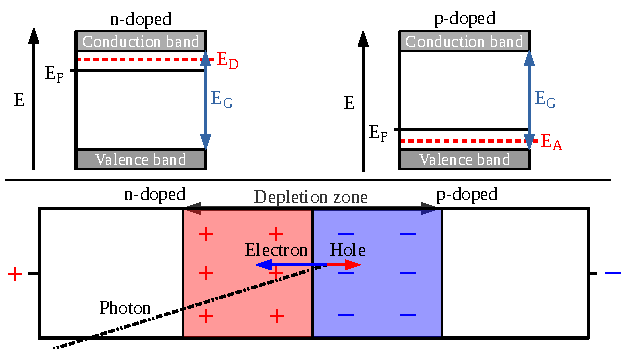
\includegraphics[width=0.7\textwidth]{PNJunction.pdf}
	\caption[Sketch of a $p$-$n$-junction]{\textbf{Sketch of a $p$-$n$-junction.} \cite{iceact:camera} In the top, the energy bands are shown for $n$-doped and $p$-doped semiconductor with the Fermi energy level $E_F$, the gap energy $E_G$, and the donor or acceptor energy level $E_D$ and $E_A$ respectively. Below, a $p$-$n$-junction is sketched. An incident photon may result in production of an additional electron-hole-pair inducing a current via avalanches.}
	\label{sipm:pn_junction}	
\end{figure}

If a photon now traverses the diode, a possible impact can ionize an atom and thus produce an electron-hole-pair. While the electron is accelerated along the electrical field it can ionize further atoms if the electric field is strong enough -- an avalanche is formed that induces a highly temperature-dependent breakdown voltage $V_\text{breakdown}$. Here, the \enquote{Geiger-mode} prefix additionally indicates that the signal is not dependent on the number of total detected photons. A quenching resistor allows to stop the avalanche and enables the cell to recover quickly. This working principle is referred to as an \textit{avalanche photo diode} (\textit{APD}). Usually, photo diodes are based on germanium (Ge) or silicon (Si). Since the band gap of silicon-based photo diodes is higher (\SI{1.12}{\electronvolt}) than for germanium-based ones (\SI{0.67}{\electronvolt}), the electrons in silicon-based photo diodes need higher energies to produce a significant photo currents. Thus, Si photo diodes generate less noise than photo diodes based on Ge. \cite{sipm:renker_lorenz} An important operation parameter of a G-APD is the over voltage $V_\text{OV}$ since many features (e.g. the gain) of G-APDs are proportional to it. It is defined as the difference of bias and breakdown voltage~\cite{sipm:renker_lorenz}
\begin{align}
	V_\text{OV} = V_\text{bias} - V_\text{breakdown}\,.
\end{align}

Basically, there are two types of G-APD cells: $p$-on-$n$ which is shown in figure~\ref{sipm:apd_cell} and $n$-on-$p$. They differ in the wavelength region they are efficient in. While $n$-on-$p$ cells are efficient for wavelengths beyond \SI{1}{\micro\meter}, the $p$-on-$n$ cells operate best in the blue and UV regime -- thus in the peak region of Cherenkov light (cf. figure~\ref{airshowers:cherenkovspectrum}).

\begin{figure}[H]
	\centering
	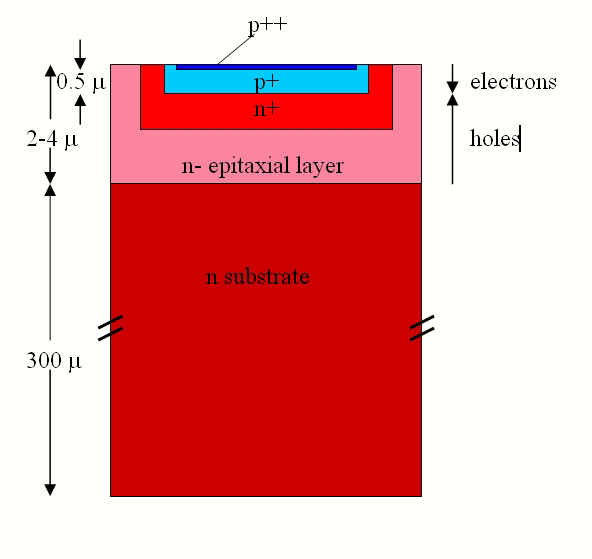
\includegraphics[width=0.5\textwidth]{APD_Cell.png}
	\caption[Sketch of a \enquote{$p$-on-$n$} G-APD cell]{\textbf{Sketch of a \enquote{$p$-on-$n$} G-APD cell.} \cite{sipm:renker_lorenz} This type is optimized to have a high photon detection efficiency in the blue and UV wavelength regime.}
	\label{sipm:apd_cell}	
\end{figure}

\begin{figure}[H]
	\centering
	\saveimageheight[width=0.34\textwidth]{SiPM_circuit.pdf}
	\begin{subfigure}[t]{0.62\textwidth}
		\raiseimage[width=\textwidth]{SiPM_picture.png}
		\subcaption{Picture of the MicroFJ-60035-TSV SiPM which is used in the \iceact camera as seen from the top (left) and the back (right). One can slightly see the fine grid of \num{22292} G-APDs with a size of $\SI{35}{\micro\meter}\times\SI{35}{\micro\meter}$ arranged on a package with the dimensions $\SI{6.07}{\milli\meter}\times\SI{6.07}{\milli\meter}$.}
		\label{sipm:iceact_sipm}
	\end{subfigure}
	\hfill
	\begin{subfigure}[t]{0.34\textwidth}
		\usebox{\savedimage}
		\subcaption{Circuit diagram of a SiPM with 12 (very few) G-APD cells in parallel connection. One can see that each cell has its own quenching resistor. The fast output is not used in the application for \iceact.}
	\end{subfigure}
	\caption[Structure of an SiPM]{\textbf{Structure of an SiPM.} \cite{sipm:datasheet}}
	\label{sipm:circuit_picture}
\end{figure}

The step from a G-APD to an SiPM is done if one now combines many G-APDs in a grid structure in parallel connection which is shown in figure~\ref{sipm:circuit_picture}. Figure~\ref{sipm:pulses} shows measured waveforms (or \enquote{pulses}) of SiPM with linear amplification. A discretization of puls heights which correspond to the number of single cell breakdowns can be observed. The amplitude $A_i$ of a standard pulse is proportional the capacitance $C$ and anti-proportional to the electron charge $q$ and the over voltage $V_\text{OV}$,~\cite{sipm:renker_lorenz}
\begin{align}
	A_i\propto\frac{C}{qV_\text{OV}}\,.
\end{align}
If now multiple cell breakdowns occur, the total pulse height just sums up over the number of triggered cells which is commonly knows as \textit{PE} (\textit{photo electron equivalent}),~\cite{sipm:renker_lorenz}
\begin{align} 
	A = \sum_{i=0}^{PE} A_i\,.
\end{align}

\begin{figure}[H]
	\centering
	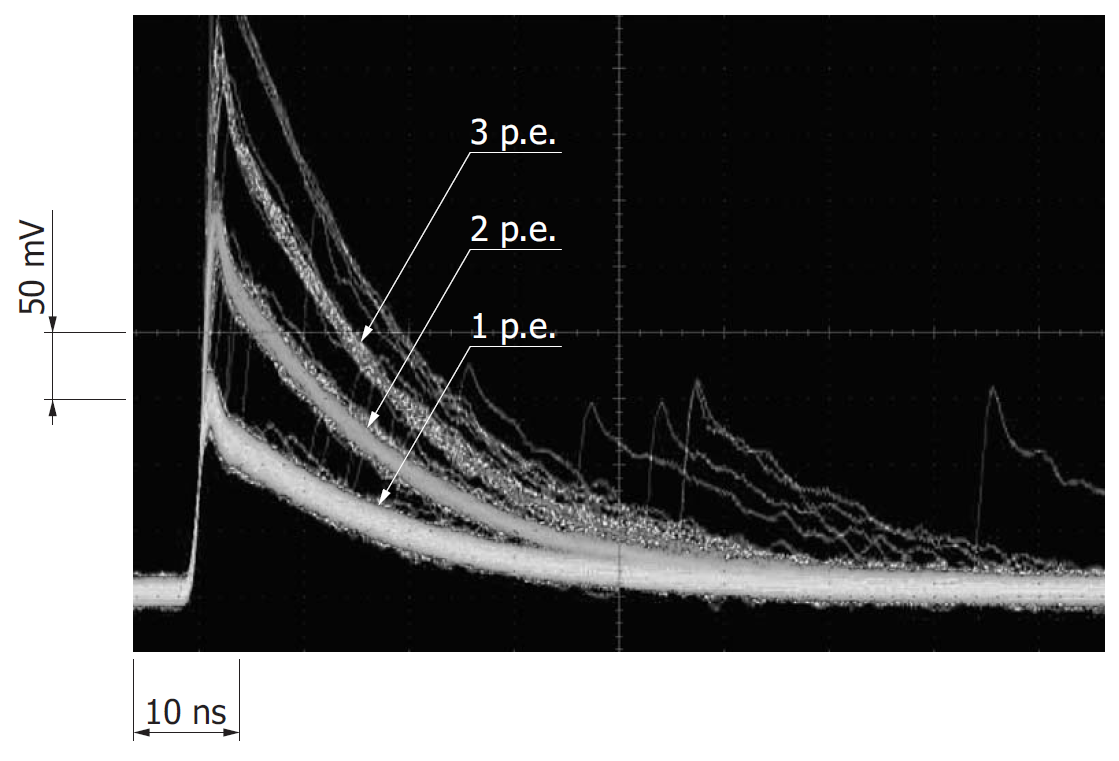
\includegraphics[width=0.7\textwidth]{SiPM_pulseplot}
	\caption[Pulse waveforms of an SiPM]{\textbf{Pulse waveforms of an SiPM.} \cite{sipm:hamamatsu_handbook} Multiple measured SiPM waveforms (\enquote{pulses}) with amplitude plotted against time. A discretization of pulse heights can be observed which is dependent on the number of single cell breakdowns marked with \enquote{p.e.} in the plot. One can see a few after pulses at later times as well.}
	\label{sipm:pulses}
\end{figure}

In addition, the pulse shape can be parameterized by a function of two exponential functions,
\begin{align}
	A(t,PE) = c\cdot PE \cdot \left(1-\frac{1}{1+\exp\left(\frac{t-t_0}{\tau}\right)}\right)\cdot\exp\left(-\frac{t-t_0}{\lambda}\right)\,,
\end{align}
where $c$ is a calibration factor, that corresponds to the amplitude of a \SI{1}{PE} pulse, $t_0$ is the starting time of the pulse, and $\tau$ and $\lambda$ are the rise and fall times respectively, which are typically in a range of $\tau=\SI{0.9}{\nano\meter}$ to $\SI{1.1}{\nano\meter}$ and $\lambda=\SI{18}{\nano\second}$ to $\SI{20}{\nano\second}$.~\cite{sipm:fact_calibration}

Moreover, figure~\ref{sipm:iceact_sipm} shows the SiPM used for the \iceact camera. It is the MicroFJ-60035-TSV SiPM by ON Semiconductor\footnote{In former theses and publications on \iceact the SiPM is called SensL J-Series 60035. Since 2018, SensL is fully integrated in the head organization ON Semiconductor which took over the sales of SensL products.}. 
It consists of \num{22292} G-APD cells with the dimensions $\SI{35}{\micro\meter}\times\SI{35}{\micro\meter}$ each. The active area is $\SI{6.07}{\milli\meter}\times\SI{6.07}{\milli\meter}$ and the package area is $\SI{6.13}{\milli\meter}\times\SI{6.13}{\milli\meter}$ which results in a fill factor\footnote{Percentage of the active area that is actually equipped with cells.} of $\epsilon_\text{fill}=\SI{75}{\percent}$. On top of the active area, a glass plate with a thickness of \SI{0.37}{\milli\meter} (cf. figure~\ref{sipm:tec_sketch}). More technical properties can be found in the data sheet~\cite{sipm:datasheet}.

\begin{figure}[H]
	\centering
	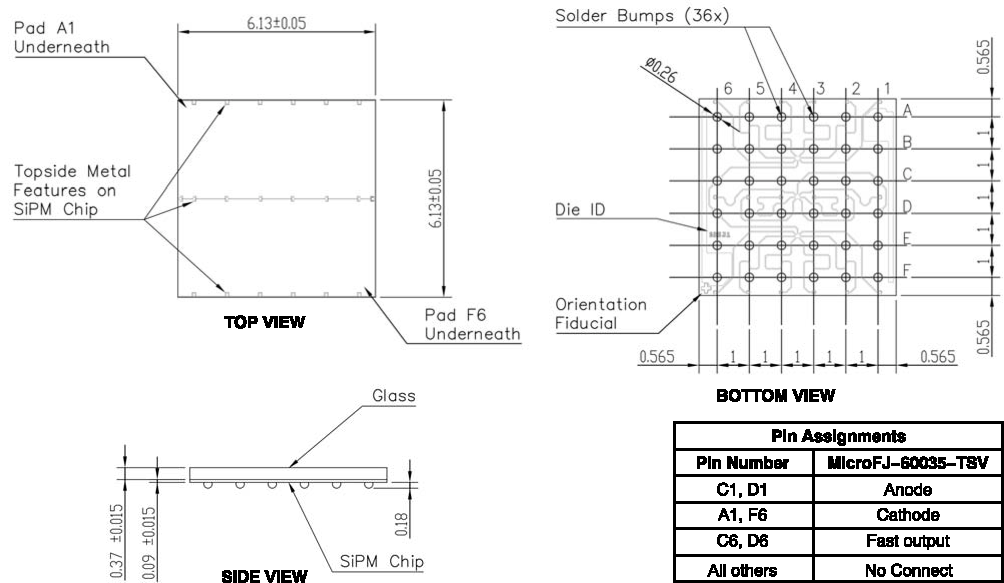
\includegraphics[width=\textwidth]{SiPM_sketch.pdf}
	\caption[Technical sketch of the MicroFJ-60035-TSV SiPM used in \iceact]{\textbf{Technical sketch of the MicroFJ-60035-TSV SiPM used in \iceact.}~\cite{sipm:datasheet} All dimensions given in \si{\milli\meter}.}
	\label{sipm:tec_sketch}	
\end{figure}

\subsubsection{SiPM Implementation in \geant with G4SiPM}

In the \iceact \geant simulation, the SiPM is implemented via the plug-in \textit{G4SiPM}~\cite{sipm:g4sipm}. It allows a convenient implementation of geometry, materials, photon detection efficiency, and many other physics and performance parameters in \geant. It is even possible to do waveform simulation with background from cross talk, after pulses, thermal noise, etc. Since the signal simulation is beyond the scope of this thesis, only the material and detection properties are of interest.

For the material properties of the \SI{0.37}{\milli\meter} thick covering glass plate on the SiPM, only the refractive index of $n = \SI{1.53}{\nano\meter}$ at a wavelength of $\lambda = \SI{436}{\nano\meter}$ is given in the data sheet~\cite{sipm:datasheet}. Since there are no detailed information about the glass, $n$ is assumed to be constant for the simulation.

The other important property is the \textit{photon detection efficiency} $PDE(\lambda,V_\text{OV})$ which is given for the over voltages $V_\text{OV}=\SI{2.5}{\volt}$ and $V_\text{OV}=\SI{6}{\volt}$ and for wavelengths $\lambda = \SI{200}{\nano\meter}$ to $\SI{900}{\nano\meter}$. In \iceact the SiPMs are operated with an over voltage of $V_\text{OV} = \SI{5}{\volt}$. Measurements in the data sheet show that the relation between over voltage and PDE is linear.~\cite{sipm:datasheet} Therefore, one gets the needed $PDE_{\SI{5}{\volt}}\coloneqq PDE(\lambda,V_\text{OV}=\SI{5}{\volt})$ by linear interpolation,
\begin{align}
	PDE_{\SI{5}{\volt}} = PDE_{\SI{2.5}{\volt}} + \frac{\SI{2.5}{\volt}}{(6-2.5)\si{\volt}} \cdot (PDE_{\SI{6}{\volt}}-PDE_{\SI{2.5}{\volt}}),
\end{align}
which is then implemented in \geant. In addition, G4SiPM takes into account, that the PDE is measured for perpendicular light incidence in air environment. By using Fresnel equations it compensates for slant photon incidences. The fill factor $\epsilon_\text{fill}$ is also divided out. \cite{sipm:g4sipm,famous:niggemann}. 
The interpolated and original PDE functions are shown in figure~\ref{sipm:pde}

\begin{figure}[H]
	\centering
	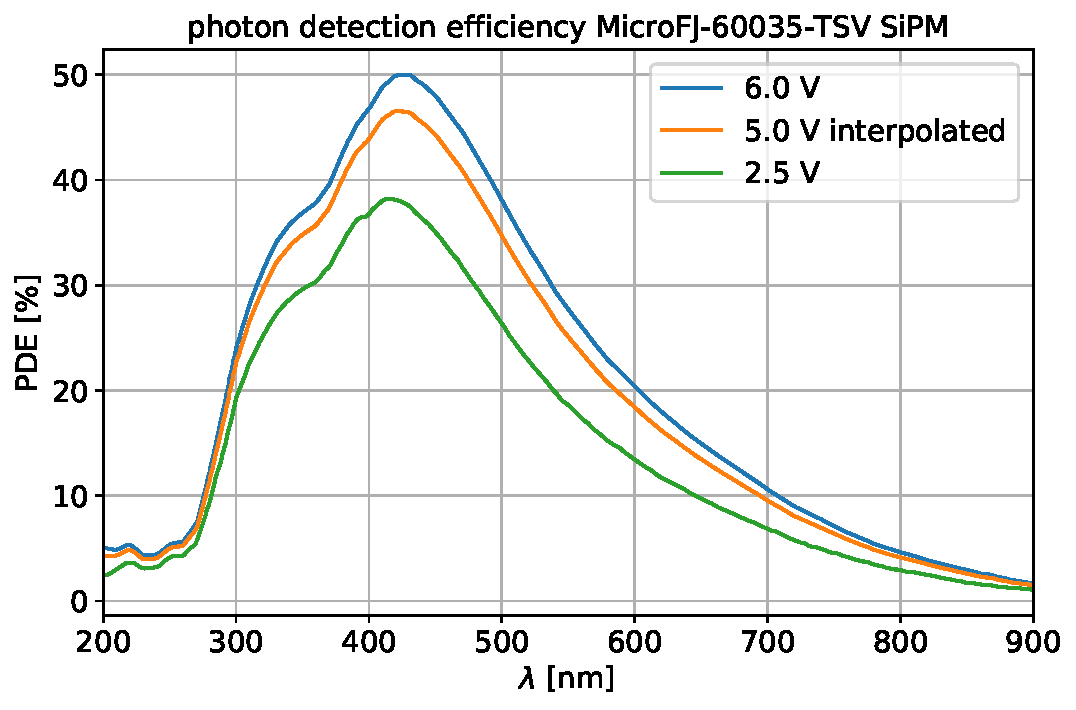
\includegraphics[width=0.7\textwidth]{material/PDE_interpolation.pdf}
	\caption[Photon detection efficiency of the MicroFJ-60035-TSV SiPM]{\textbf{Photon detection efficiency of the MicroFJ-60035-TSV SiPM.} The data for over voltages of \SI{6}{\volt} and \SI{2.5}{\volt} is taken from~\cite{sipm:datasheet}, the curve for \SI{5}{\volt} -- which is used in the \geant simulation -- is interpolated linearly.}
	\label{sipm:pde}	
\end{figure}
